\section{Direct Mapping (DMap)}
%\section{System design}
\label{sec:design}
In DMap, each GUID$\rightarrow$NA mapping is stored in a set of ASs. %We propose to use the route-able address space announcements made by each AS as a basis for assigning GUIDs to ASs. 
Each GUID is directly hashed to existing network addresses and its mapping is thus stored within the ASes corresponding to these network addresses. %through routing updates,i.e., which are BGP updates in today's Internet. The novel design decision of using the announced address space to distribute GUIDs has the following benefits: (1) low latencies due to \emph{single overlay hop} in both update and lookup, (2) very little state information to maintain by leveraging the existing routing structure, and (3) proportional assignment of GUID mappings to hosting ASs due to randomization.

\subsection{Overview of DMap}

%In this section, we describe the scheme of directly hashing to an IP address and enumerate the implementation issues involved along with our solutions for them. Alternatives to using the IP space are discussed in Section ?

In designing our mapping method, we strive to minimize update/lookup latencies as well as the amount of state information that needs to be maintained.  We achieve these goals by leveraging the globally available BGP reachability information to distribute the GUID$\rightarrow$NA mappings among all the participating ASs. In our scheme, DMap first hashes a GUID to an existing network address, and then stores its GUID$\rightarrow$NA mapping within the AS that announces this network address. This results in exactly a single overlay hop for all the update/lookup requests without introducing any additional state information on each router.  Next, we look at an example to illustrate this approach. In this example, we assume the usage of the existing IP address space, but we note that the same technique can be easily extended to any future addressing scheme such as IPv6, AIP~\cite{andersen} or HIP~\cite{moskowitz}.
   
% \vspace{-0.25in}
% \hspace{0.1in}
Let us suppose host $X$, with GUID $G_x$, is attached to NA $N_x$. $X$ first sends out a \emph{GUID Insert} request, which is captured by the border gateway router in its AS. The border gateway router then applies a predefined consistent hash function on $G_x$ and maps it to a value $IP_x$ in the IP space.  Based upon the IP prefix announcements from its BGP table, the border gateway router finds out which AS owns $IP_x$ and sends the $G_x\rightarrow N_x$ mapping to that AS.  Later, suppose host $Y$ wishes to look up the current locator for GUID $G_x$. $Y$ sends out a \emph{GUID Lookup} request. After the request reaches $Y$'s border gateway router, the border gateway runs the same hash function to identify the AS that stores the mapping. Every time when $X$ changes its association and connects to a different AS, it needs to update its mapping by sending out a \emph{GUID Update} request. Update requests are processed similarly as insert and lookup requests.

Using the above approach, a GUID's mapping is hashed to a random AS, without considering the locality between the GUID and its lookup requests. This lack of locality may potentially lead to unnecessarily long lookup latencies.  Thus, instead of storing a mapping at only one AS,  we consider having $K$ replicas of the same mapping stored at $K$ random ASs. Having $K$ replicas can significantly reduce the lookup latency as the requesting node can choose the closest replica (e.g., based upon the hop count between itself and the hosting ASs). Meanwhile, it will not have a big impact on the update latency as we can update the replicas in parallel.
With $K$ mapping replicas, the lookup latency becomes the shortest latency among the $K$ ASs, while the update latency becomes the largest among the $K$ ASs. Figure~\ref{fig:design} illustrates an example update and lookup process with $K = 3$. Finally, we note that important DMap parameters, such as which hash functions to use and the value of $K$, will be agreed and distributed before hand among the Internet routers.

\begin{center}
        %\vspace{-0.2in}
        \begin{figure}[t]
            \centering
            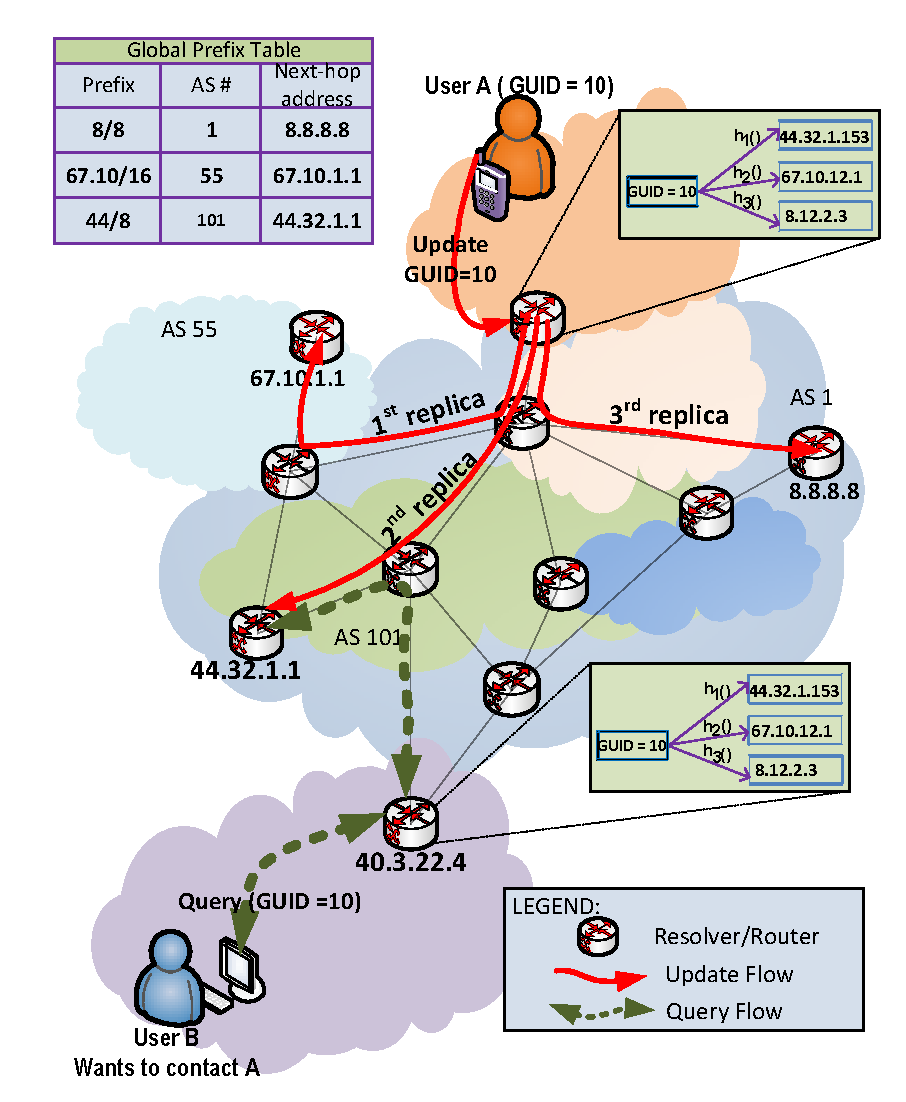
\includegraphics[width=0.4\textwidth]{figures/designV2.eps}
            \caption{DMap with K=3 independent hash functions}
            \label{fig:design}
            \vspace{-0.2in}
        \end{figure}
    \end{center}

\vspace{-0.2in}
Compared to other mapping schemes, one distinct feature of DMap is the direct participation of network routers in storing GUID$\rightarrow$NA mappings and in responding to updates and lookups. DMap does not require any additional state information as the IP reachability information is already made available by the BGP routing protocol.  In addition, we note that unlike many recent proposals~\cite{farinacci-alt,jen,jakab,mathy}, DMap does not distribute GUID mappings based on the assumption of the aggregate-ability of
the GUID space.  Our scheme is suitable for flat address spaces, which has been pointed out as a desirable feature for the Future Internet~\cite{andersen,moskowitz}.

\subsection{Handling Unallocated Network Addresses}
\label{subsec:ip_hole}

DMap hashes a GUID to an IP address, and stores the GUID mapping in the AS that announces this IP address.  Due to fragmentation in the IP address space, it is possible that the hashed IP address is not announced by any AS. This problem is referred to as the \emph{IP hole problem}. To understand the extent of this problem, we take a close look at today's IP address space. At present, 86\% of the $2^{32}$ IP addresses available in IPv4 are allocated to various entities~\cite{dix-ie}; the rest are reserved for other purposes including multicast, limited multicast, loopback address, broadcast, etc. Among the allocated addresses, 63.7\% of them are announced by one of the ASs. This leads to an overall 55\% announcement ratio over the entire IPv4 address space, which results in a 45\% chance that a randomly hashed $IP_x$ will belong to the set of unannounced addresses.
% or, IP holes.

 %While the technique produces the benefit of low latency naming look up and update since it only requires one overlay hop to reach the resolver, it suffers to the discontinuity of the address space. Since the hashed value of a GUID is equally distributed over address space, there is a probability that the hashed value falls into the address block that no organization have announced. We call the problem is \emph{IP hole effect}. % might need to change the name
%        For example, in current Internet, while there are $2^{32}$ possible IP addresses for IPv4, only 86\% of them are allocated to organizations. The rest are reserved for various purposes including multicast, limited multicast, loopback address, broadcast, etc. Among those allocated address, only 63.7\% of them are announced by organizations. As the result, the percentage of announced IP address is only 55\%[cite IP hole data] over the whole 32-bit IP space, giving the probability for a hashed result falling into one of the unannounced address is 45\%.

We address the IP hole problem by finding a deputy AS through rehashing if the IP address after the first hash falls into a hole. After $M-1$ rehashes, if the resulting address still falls into an IP hole, we pick the deputy AS as the one that announces the IP address that has the minimum \emph{IP distance} to the current hashed value. Given two k-bit addresses, A and B, their IP distance is defined as:
\begin{center}  %\vspace{-0.1in}
$IP\_distance_{[A,B]} = \displaystyle\sum\limits_{i=0}^{k-1} |A_i - B_i|*2^{i}.$ \end{center}
We further define the IP distance between an address and an address block as the minimum IP distance between that address to all addresses in the block. In this way, we can guarantee that a deputy AS can always be found.

There is a concern that the above method may introduce load imbalance among ASs: the AS that announces an IP address that is adjacent to a large set of reserved addresses (thus unannounced) may become a popular deputy AS and needs to store a large number of mappings. Fortunately, the probability of reaching an IP hole after $M$ hashes decreases rapidly with increasing $M$.
For instance, this probability is as low as 0.034\% for $M=10$. As a result, the chances that we need to resort to the ASs that announce the IP addresses with the minimum IP distances to the holes are very low.

Algorithm \ref{alg:rehashing} summarizes the steps taken by the border gateway to deal with the IP hole problem. Since hashing, rehashing and prefix matching processes are done locally by the border gateway, these operations introduce very little delay to the network.
       {
        \begin{algorithm}
            \small
            \SetAlFnt{\small\sf}
            \SetKwData{numbtry}{number\_of\_tries}
            \SetKwData{nearestPrefixID}{nearestPrefixID}
            \SetKwData{mindist}{min\_distance}
            \SetKwData{result}{result} %declare
            \SetKwFunction{lpm}{Longest\_Prefix\_Matching}
            \SetKwFunction{ipd}{IP\_distance}
            \SetKwFunction{findClosestPrefix}{find\_closest\_prefix} 
            \SetKwFunction{Hash}{hash}
            \SetKwInOut{Input}{input}
            \SetKwInOut{Output}{output}
            \Input{GUID - the $GUID$ to be hashed \\ \hspace{0.5cm}$M$ - maximum number of rehashing}
            \Output{An address guaranteed to be found in prefix table}
            \BlankLine
            $\numbtry \leftarrow 0 ;$\;
            $\result \leftarrow \Hash{GUID};$\;
            \While{ ($\numbtry < M $)}{
                \If{\lpm{\result} $>$ 0}{
                \Return \result; //ended here if found\;
                }
                 {// no prefix was found}\;
                $\result \leftarrow \Hash{\result}; $\;
                $\numbtry \leftarrow \numbtry+1 ;$\;
            }
            //No match found after M hashes\;            
	         \nearestPrefixID = findNearestPrefix(\result); 
%            $\mindist \leftarrow 2^{32}$;\;
%            \lForEach{prefix $i$ in the Prefix Table}{\;
%               \If{\ipd{\result,prefix $i$} $<$ \mindist}{
%                   \mindist $\leftarrow$ \ipd{\result to the prefix};\;
%                }
%            }
			\BlankLine
            \Return An address in \nearestPrefixID;
         \caption{Hashing GUID to address space} \label{alg:rehashing}
        \end{algorithm}\vspace{-12pt}
        }

When extending DMap to other network address schemes, such as IPv6, we need to rethink how we deal with the IP hole problem as these network address spaces may have substantially more holes than used address segments. To address such sparse address spaces, we propose to use a two-level indexing method to index each announced address segment: bucket ID and segment ID within that bucket. Suppose we have $N$ buckets, each with a capacity of $S$ segments. We make $N$ large so that $S$ can be kept small. Given a GUID, we run two hash functions, the first one mapping the GUID to bucket ID, and the other one mapping the GUID to the segment ID. Figure \ref{fig:bucketing} illustrates the bucketing scheme.

 \begin{center}
        %\vspace{-0.2in}
        \begin{figure}[t]
            \centering
            \includegraphics[width=0.5\textwidth]{figures/bucketting.eps}
            \caption{Bucketing scheme handling non-contiguous address space issue}
            \label{fig:bucketing}
            \vspace{-0.2in}
        \end{figure}
    \end{center}

%\subsection{Replication}
%\label{subsubsec:replication}
%To enhance DIHT's reliability and further reduce access latencies, we increase the number of resolvers responsible for each mapping entry by having the border gateways employ $K$ parallel hash functions at the time of update and query. During insertion or update, the border gateway applies Algorithm~\ref{alg:rehashing} $K$ times using independent hash functions on each iteration to obtain $K$ valid addresses. The mapping is stored in all the $K$ ASs responsible for the resulting addresses, thus creating storage replicas for each entry in the mapping table. To lookup a mapping entry, the gateway router selects the closest AS (in terms of path cost obtained from the BGP table) among the $K$ ASs that maintain the required mapping.
%After receiving the query, the border gateway applies Algorithm \ref{alg:rehashing} for K times with K different hashing functions to obtain K valid resolvers's addresses. Among these K resolver, It looks at the prefix table to choose the closest one. The notion of `closest' can be measure in terms of BGP distance (e.g. hop counts), or IP distance as mentioned in the previous subsection.
%This replicating technique leads to two important benefits - reduced lookup latencies and increased resilience to random failures. Firstly, with randomized replication, a gateway is more likely to find a nearby AS which stores the required mapping. We show in Section~\ref{sec:evaluation} that as $K$ increASs from 1 to 5, the 95th percentile lookup latency reduces from 202ms to 91ms. Secondly, as the number of replicas increASs, the resilience of the system is also greatly improved as the probability of two distant routers failing simultaneously is very low. Figure \ref{fig:design} illustrates an example of the update and query process with $K=3$. Finally, we note that this method interleaves the mapping replicas between ASs in contrast to exact replication of all the mappings from one AS to another, thus adding resilience random failures.

%The improvement in latency and reliability, however, comes with an increased storage requirement and enhanced complexity in the update process. A careful analysis based on the bounds on requirements and capabilities of the network is thus required to select an appropriate value for $K$.
        %Having too many replica can leads to increase in update delay and introduce addional network traffic. As the result, we need to carefully choose value for K in our design.
        %While it is obvious to see the query latency reduces as higher K is used, K can not be arbitrarily increased due to update propagation delay. Specifically, propagation delay for each update equals to the largest update delay to individual resolver, assuming the gateway simultaneously updates to all resolvers at once. Hence the inherent trade of between query latency and update latency must be taken into account when K is being used as the knob to tuning the network's performance

\vspace{-0.3in}
\subsection{Spatial Locality and Local Replication}
\label{sec:locality}

The main advantage of DMap lies in its simplicity: hashing a GUID to a random AS.  However, this random placement ignores locality, and so may degrade performance.  Having multiple replicas partially addresses this problem, but it still has the inherent problem of a direct hashing scheme: the GUID mappings are stored at faraway ASs when the host and requestor are close to each other.  Thus, we enhance the baseline DMap for an expected common case of when a requesting node is attached to the same AS as the GUID that it is resolving.  To leverage this \emph{spatial locality}, DMAP stores an additional replica of a GUID mapping at its attached AS.  When a host registers/updates its GUID, it creates/updates a local copy (at its attached AS) in addition to creating/updating the $K$ ``global'' copies. When a node needs to lookup a GUID, it sends out a local and a global lookup simultaneously.  When the host and the requester are from the same AS, the local request should lead to significantly reduced lookup latency.

% \begin{center}
%        \vspace{-0.2in}
%        \begin{figure}[t]
%            \centering
%            \includegraphics[width=0.5\textwidth]{figures/localCache.eps}
%            \caption{Local replication enhancement}
%            \label{fig:local_rep}
%            \vspace{-0.2in}
%        \end{figure}
%  \end{center}
\subsection{Inconsistent GUID$\rightarrow$NA Mappings}
\label{sub:inconsistency}

\subsubsection{BGP Churn} Since a change in the prefix announcements directly influences DMap, we analyze the potential effects of BGP churn. A long term study of BGP churn evolution~\cite{elmokashfi} shows that a major reason for churn in the BGP tables is router configuration mistakes or other anomalies. Changes in prefix announcements occur when an AS withdraws a previously announced prefix or announces a new prefix.  The actual rate of new prefix announcement and prefix withdrawal is small, with the former dominating the latter.

When an AS withdraws a certain prefix, all the mappings previously hosted by the AS whose GUIDs are hashed to the withdrawn IP addresses will become unaccessible, resulting in what we call \emph{orphan mappings}.   To address this problem, we let the withdrawing AS run the IP hole protocol to find a deputy AS for these mappings before withdrawing. It sends  a \emph{GUID insert messages} to the deputy AS and deletes its own copy of the mapping. Subsequent queries will then hit an IP hole. Following the same IP hole protocol, they will reach the deputy AS and find the mapping.

Announcing new prefixes can also result in orphan mappings. The GUIDs that were originally hashed to these IP addresses had followed the IP hole procedure to a ``deputy'' AS, and announcing these addresses now can make the mappings on the deputy AS orphan mappings. As a result, queries that reach the announcing AS will not find the mappings, while the mappings on the deputy AS become inaccessible. To solve this problem, when the announcing AS receives a query and finds the mapping missing, it sends a \emph{GUID migration message} to the deputy AS to relocate the mapping to itself. This operation could cause a negligible one-time overhead, which only occurs for the first query after the announcement.


%{\bf Need to mention Latency vs. BGP churn result here}

%In the latter case, where an AS announces new prefix, it becomes much more tricky. There will be queries that go to the AS with GUID that does not stored on any of the AS's border gateways, since it is stored in other AS that is behind the current AS in the hashing chain. In such cASs, the border gateway of the newly announced AS has to (1) first verify that he is on the hash chain of of that GUID, which can be done simply by applying K hash functions, m times for each on the given GUID. After positively confirmed, (2) the border gateway must go the the address right after him on the hashing chain to get the GUID and (3) inform that the mapping now becomes orphan to the AS right behind him so that the behind AS can start collecting garbage, certainly after a verification. The border gateway then stores the mapping on to permanent memory in order to be ready for the next query of the same GUID. Note that to reduce the user visibility on prefix change, the border gateway can in parallel issues P query to P resolvers, with $P<K$.

\subsubsection{Mobility} Mobility can also lead to inconsistencies in DMap. Suppose host $X$, with GUID $G_x$, is connected to AS $A$. As a result, DMap has the mapping $(G_x : A)$. Then suppose $X$ moves to AS $A'$ at time $t_0$, and its mapping will be updated to  $(G_x : A')$ at time $t_1$.  While we expect $t_1-t_0$ to be small, it is possible for a querying node to get the old mapping right after X has moved.  The querying node will then be unable to communicate with $X$.
In this case, the querying node should mark the mapping as obsolete, and 
keep checking until it receives an updated one.

\subsubsection{Router Failure} An AS can lose part or all of its mappings due to router failure. This is a rare event, but we need to address the resulting complication.  If a lookup request reaches an AS, but cannot find the mapping due to this problem, the requestor will wait for a timeout. Following the timeout, the requestor will contact the next mapping replica (remembering we have $K$ replicas in total). We note that the probability for $K$ Internet routes to fail at the same time is extremely low, and thus our replication strategy also improves system resilience and reliability.
